% BÀI TOÁN HÌNH HỌC - BAI_HINH_20 (TRÍCH ĐỀ 20)
\begin{ex}
Cho đường tròn (O;R) và dây cung AB < 2R. Gọi H là trung điểm của AB, đường thẳng HO cắt đường tròn (O) tại hai điểm C và D (C thuộc cung nhỏ AB). Điểm M thuộc đoạn AH (M khác A và H), tia CM cắt đường tròn (O) tại điểm thứ hai là N. Gọi I là giao điểm của hai đường thẳng DN và AB, K là giao điểm của hai đường thẳng CI và DM.
	\begin{enumerate}
		\item[a)] Chứng minh rằng: Bốn điểm I, A, M, N thuộc 1 đường tròn.
		\item[b)] Chứng minh rằng $CM \cdot CN = CK \cdot CI$ và M là tâm đường tròn nội tiếp tam giác HKN.
	\end{enumerate}
\loigiai{
{
	\begin{center}
		
		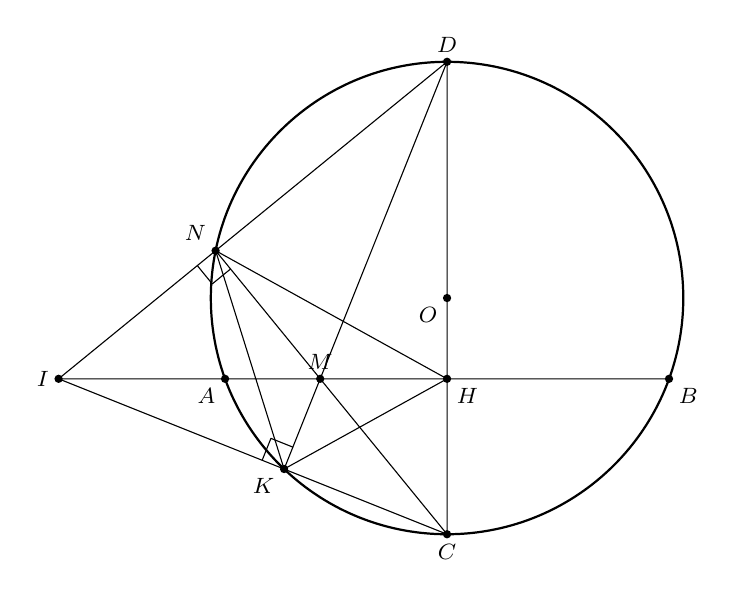
\begin{tikzpicture}[line join = round, line cap=round,>=stealth,font=\footnotesize,scale=1]
			\usetikzlibrary{calc,intersections,angles} % Added intersections
			% Def
			\def\r{3}
			
			% Coordinates
			\coordinate (O) at (0,0);
			\coordinate (D) at (90:\r);    % D on positive y-axis
			\coordinate (A) at (-160:\r);  % A in Q3
			\coordinate (B) at (-20:\r);   % B in Q4
			\coordinate (C) at (-90:\r);   % C on negative y-axis
			
			% H is midpoint of AB
			\coordinate (H) at ($ (A)!0.5!(B) $);
			
			% I such that vector IA = 3/8 vector AB
			% vec(I) = vec(A) - 3/8 * (vec(B) - vec(A)) = 11/8*vec(A) - 3/8*vec(B)
			\coordinate (I) at ($ 11/8*(A) - 3/8*(B) $);
			
			% N is projection of C onto ID
			\coordinate (N) at ($ (I)!(C)!(D) $);
			
			% K is projection of D onto IC
			\coordinate (K) at ($ (I)!(D)!(C) $);
			
			% M is intersection of DK and NC
			% Define paths for intersection
			\path[name path=DKline] (D) -- (K);
			\path[name path=NCline] (N) -- (C);
			% Find intersection
			\path[name intersections={of=DKline and NCline, by=M}];
			
			% Draw
			% Draw circle (O,r)
			\draw[thick] (O) circle (\r);
			
			% Draw paths I-D-C-I (triangle IDC)
			\draw (I) -- (D) -- (C) -- cycle; 
			
			% Draw path I-B-H-N-K-H
			\draw (I) -- (B) -- (H) -- (N) -- (K) -- (H);
			
			% Draw N-C
			\draw (N) -- (C);
			
			% Draw D-K
			\draw (D) -- (K);
			
			% Fill points
			\fill (O) circle (1.5pt);
			\fill (D) circle (1.5pt);
			\fill (A) circle (1.5pt);
			\fill (B) circle (1.5pt);
			\fill (C) circle (1.5pt);
			\fill (H) circle (1.5pt);
			\fill (I) circle (1.5pt);
			\fill (N) circle (1.5pt);
			\fill (K) circle (1.5pt);
			\fill (M) circle (1.5pt);
			
			% Node points (old style)
			\node[below left] at (O) {$O$};
			\node[above] at (D) {$D$};       % D is (0,3)
			\node[below left] at (A) {$A$};  % A is approx (-2.8, -1.0)
			\node[below right] at (B) {$B$}; % B is approx (2.8, -1.0)
			\node[below] at (C) {$C$};       % C is (0,-3)
			\node[below right] at (H) {$H$};       % H is approx (0, -1.0)
			\node[left] at (I) {$I$};         % I is approx (-4.9, -1.0)
			\node[above left] at (N) {$N$}; % N is on ID, depends on projection
			\node[below left] at (K) {$K$};  % K is on IC, depends on projection
			\node[above] at (M) {$M$};       % M is intersection, position varies
			
			% Ky hieu goc vuong (old style)
			% CN is perpendicular to ID
			\pic[draw, angle radius=3mm]{right angle = C--N--I}; % or C--N--D
			% DK is perpendicular to IC
			\pic[draw, angle radius=3mm]{right angle = D--K--I}; % or D--K--C
			
			\end{tikzpicture}
				
	\end{center}
}
\end{ex}
